En este capítulo se especifican las pruebas a las que se ha sometido el proyecto,
y las configuraciones y herramientas necesarias para poder llevarlas a cabo.

\section{Estrategia}

La estrategia de pruebas seguida es una serie de pruebas exhaustivas y
completas, llevadas a cabo cada vez que se modificaba algún componente
importante y revisando todas las funcionalidades repetidas veces en entornos
asegurados.

\section{Entorno de pruebas}

Se distingue entre el entorno de pruebas de la API, que va a ser desplegada en
un único servidor, y el de la aplicación móvil, que puede ser desplegada en
multitud de dispositivos.

\subsection{API}

Para la utilización de entornos de prueba se ha optado por Vagrant, una
herramienta capaz de crear y configurar ambientes virtuales de manera sencilla,
reproducible y portátil. Permite desplegar el sistema necesario en una máquina
virtual tantas veces como se necesite y desde cualquier equipo que tenga Vagrant
instalado.

Esta herramienta tiene la ventaja de que permite crear las reglas de
configuración una única vez y reutilizarlas en casa ocasión, sin tener que volver
a desplegar el mismo sistema desde cero cada vez que se cambie de equipo.

El archivo principal de Vagrant es \texttt{Vagrantfile} que contiene la
configuración básica que se leerá cada vez que se ejecute un comando de Vagrant.

Vagrant permite utilizar multitud de plataformas de configuración, como Chef,
Puppet o Ansible. Hemos optado por esta última. Para poder utilizar Ansible para
definir las reglas de configuración del sistema hay que añadirlo a este archivo
de configuración:

\begin{minted}{bash}
  config.vm.provision "ansible" do |ansible|
    # ansible.sudo = true
    ansible.extra_vars = { ansible_ssh_user: 'vagrant',
    remote_user: 'vagrant', port_arg: PORT_NUMBER}
    ansible.raw_ssh_args = ["-o UserKnownHostsFile=/dev/null"]
    ansible.playbook = "provisioning/playbook.yml"
  end
\end{minted}

El archivo \texttt{playbook.yml} describe las reglas a seguir cada vez que se
despliegue un sistema. Este archivo puede contener tareas directamente o
llamadas a conjuntos de tareas, como es el caso.

\begin{minted}{bash}
---
- hosts: all
  vars_files:
    - vars.yml
  roles:
    - system
    - nginx
    - postgresql
    - django
    - gunicorn
    - supervisor
    - deploy
\end{minted}

Puede verse que se carga un archivo de variables y luego cada una de los
conjuntos de tareas. Se han organizado en función de los subsistemas que se
despliega con cada conjunto.

Una tarea puede tener los sigueintes atributos definidos en Yaml:
\begin{itemize}
\item \texttt{name}: nombre descriptivo de la tarea
\item \texttt{become}: ejecutar la tarea como otro usuario (si no se especifica,
  \texttt{become\_user}, se ejecutará como \texttt{root})
\item \texttt{command}: órden a ejecutar tal y como se escribiría en la terminal
\item \texttt{apt}: instalación de paquetes mediante \texttt{apt-get}
\item \texttt{git}: utilización de repositorios Git (clonado, pull, ...)
\item \texttt{stat}: utilización de archivos (creación, cambio de permisos,...)
\item \texttt{template}: utilización de plantillas (archivos con variables)
\end{itemize}

Por ejemplo, la configuración básica del sistema se encarga de:
\begin{enumerate}
\item Actualizar los paquetes del sistema.
\begin{minted}{bash}
- name: update and upgrading packages
  become: yes
  apt: update_cache=yes upgrade=safe
\end{minted}

\item Instalar los paquetes de python:
\begin{minted}{bash}
- name: install software-properties-common
  become: yes
  apt: pkg={{ item }} state=latest
  with_items: 
    - software-properties-common
    - python-setuptools
    - python-dev
- name: install pip3
  become: yes
  apt: pkg={{ item }} state=latest
  with_items:
    - python3-pip
    - python3-setuptools
- name: install pip again with easyintall
  become: yes
  command: python3 -m easy_install pip
\end{minted}

\item Instalar las dependencias de psycopg2:
\begin{minted}{bash}
- name: install dependencies for psycopg2
  become: yes
  apt: pkg=python-psycopg2 state=latest install_recommends=yes
\end{minted}
  
\item Instalar Git:
\begin{minted}{bash}
- name: install git
  become: yes
  apt: pkg=git state=latest
\end{minted}

\item Clonar el repositorio del proyecto:
\begin{minted}{bash}
- name: clone rep from GitHub
  git: accept_hostkey=true repo="{{ project_git_url }}"
       dest="~/{{ name_project }}"
\end{minted}

\item Asegurar la configuración supervisor:
\begin{minted}{bash}
- name: ensure supervisor is up to date
  become: yes
  apt: pkg=supervisor state=latest
- stat: path=/etc/supervisor/conf.d/{{ name_project }}.conf
  register: supervisor_conf
- name: ensure project stop
  when: supervisor_conf.stat.exists == True
  become: yes
  supervisorctl: name={{ name_project }} state=stopped
\end{minted}
  
\end{enumerate}

En el repositorio drf-vagrant-config puede verse la configuración completa.

Entonces, para ejecutar un entorno de pruebas aceptable, tan sólo hay que
ejecutar sobre la raíz del directorio \texttt{drf-vagrant-config}:

\begin{minted}{bash}
$ vagrant up
\end{minted}


\subsection{Aplicación móvil}

Para las pruebas sobre la aplicación móvil, dado que se realizan directamente
sobre el sistema en producción, el entorno coincide con los dispositivos de
prueba dispuestos en la sección~\ref{sec:costes} y diversos entornos variados de
otros probadores, según se especificará más adelante.


\section{Roles}

Se presentan dos roles principales necesarios para la ejecución de las pruebas.

\subsection{Probador principal}

El desarrollador del proyecto es el principal probador del sistema y de la
aplicación. Por un lado, es el encargado de desplegar y testear en el entorno
de prueba de la API, teniendo la obligación de revisar las acciones y resolver
los conflictos que surjan. Además, ha de probar la aplicación móvil como si
fuera un usuario final más.

\subsection{Probadores externos}

Para más versatilidad, se ha utilizado el programa de betas de Google, a través
del cual se permite subir una aplicación móvil al Play Store, de forma que tan
sólo los usuarios a los cuales se les permita el acceso podrán descargar y
probar la aplicación.

\begin{figure}[htbp]
  \centering
  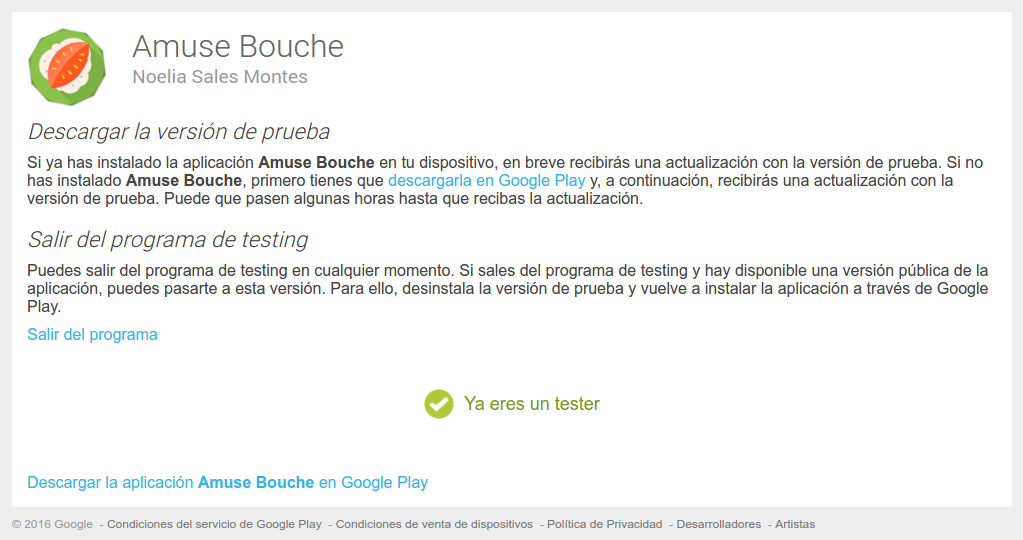
\includegraphics[width=\textwidth]{cap7/img/google-beta}
  \caption{Google Beta}
  \label{fig:google-beta}
\end{figure}

Los probadores externos han opinado sobre todos los aspectos de la aplicación,
incluyendo la interfaz de usuario, la usabilidad y la funcionalidad de esta.
Opiniones que siempre han sido teniedas en cuenta y han servido para mejorar
la aplicación.

Así, tenemos la seguridad de que la aplicación ha sido probada en dispositivos
muy variados.


\section{Pruebas funcionales}

\subsection{Pruebas de sistema}

Las pruebas de sistema, que buscan asegurar que el sistema cumple con todos
los requisitos establecidos, se desarrollaron de forma continua a medida que iba
avanzando el proyecto.

En cada iteración, las pruebas se ejecutaron sobre el entorno especificado y se
conectaron dispositivos para comprobar cómo se comportaba en condiciones
reales.

\subsection{Pruebas de aceptación}

Para verificar que el producto estaba listo para el paso a producción, se hizo
un despliegue en un servidor real y se abrió la beta de Google para confirmar
que el sistema funciona con varios usuarios usando la aplicación móvil
simultáneamente. El servidor ha permanecido online desde principios del mes de
julio hasta la fecha.


\section{Pruebas no funcionales}

Las pruebas no funcionales buscan verificar aspectos del proyecto más allá de su
funcionalidad, como la seguridad.

\subsection{Pruebas de seguridad}

Las pruebas de seguridad sirven para verificar que la información de los
usuarios y las áreas privadas de la API son seguras. Entre las pruebas que se
realizaron se encuentran las siguientes:
\begin{itemize}
\item Se intentó acceder a URLs de la zona de usuarios autenticados sin tener
  un token válido. Por ejemplo, al intentar acceder a la URL
  \url{http://amuse-bouche.noeliarcado.es/auth/me/} da un error 403 con la
  siguiente respuesta:
  \begin{minted}{bash}
{"detail":"Authentication credentials were not provided."}
  \end{minted}

\item Se intentó iniciar sesión con credenciales inválidas. La petición devuelve
  un error 403 con el siguiente mensaje:
  \begin{minted}{bash}
$ curl -X POST http://amuse-bouche.noeliarcado.es/auth/login/
    --data 'username=test&password=test'

{"non_field_errors":["Unable to login with provided credentials."]}
  \end{minted}

  
\end{itemize}

\subsection{Verificación de la calidad del código}
